% PARKED 4 Nov 2026, at the researcher's decision: Chapter 10's B3 section as it stood, with the excitable-model
% results (FitzHugh--Nagumo, Izhikevich and the kernel, judged by held-out cycles) and their figures. The models
% fit the drop cycles, but they fit fake cycles cut from noise about as well, so the fits say nothing specific
% about fungal signals. The 4 Nov follow-up on the longest trains (van der Pol, Morris--Lecar, PRCs) is in
% docs/rq_roundA_2/findings/b3-long-trains-2026-11-03.md and docs/thesis/data/ch10_fhn_long/.
% This file is NOT input by main.tex. Chapter 10 keeps the restitution half. To restore the models, paste the
% parts back into chapters/10_roundb.tex's B3 section (its labels fig:b3track, fig:fhnfit, fig:fhn live only here).

\section{Modelling common motifs}
\label{sec:rb_models}

\begin{instructions}
\textbf{B3}: does an excitable-system model describe drop cycles better than a fall plus smooth recovery? The first fits
(below) answer ``not on shape alone'': the FitzHugh--Nagumo model fits smoothed noise as well as it fits the recorded
cycles. Decided 28 Oct (Round 5 Q1): run both of the tests below.
\begin{itemize}
  \item \textbf{The restitution test} (cardiac electrophysiology): does a drop's recovery shorten when the gap before
        it was short? It needs no model fit. Recovery times come from Event shape and gaps from Intervals. The null
        shuffles the gaps within each sequence. Primary data: trains (the Library's sequences and the
        \texttt{chain\_cycles} chains). Secondary: consecutive events in the drop-detector census.
  \item \textbf{Per-cycle model tracking} on the three fitted sequences and the long chains, with four models: the fall
        plus recovery, FHN excitable and oscillatory, and Izhikevich (firing patterns; the spiking-families framing).
        Models are judged by held-out-cycle prediction against the mean of the other cycles, not by R$^2$. Parameter
        drift is tested against shuffled cycle order. Every number is set beside the same fit on fake cycles.
\end{itemize}
Hindmarsh--Rose (bursting), Morris--Lecar (type I/II) and van der Pol (relaxation) are not fitted; name them in
Chapter~\ref{ch:discussion} as further candidates. The fitter stays backend computation reading the site's cycle stacks
(Round 5 Q2), in \src{Pipelines/fhn/}. Figures go to \src{docs/thesis/data/ch10_fhn/}. The findings go to
\src{docs/rq_roundA_2/findings/fhn-fit-2026-10-26.md} and \src{docs/rq_roundA_2/findings/b3-restitution-tracking-2026-10-28.md}.

Present the phase response curves in the manner of Wilshin, Kvalheim and Revzen \cite{wilshin2024prc}: the
phase-coloured limit cycle with isochron ticks, and the PRC against phase. Say plainly that these are PRCs of the fitted
model. No perturbation experiment was made, and the paper's lesson applies: the voltage PRC depends on which hidden
variable is held constant.
\end{instructions}

\begin{instructions}
First results (\src{docs/rq_roundA_2/findings/fhn-fit-2026-10-26.md}; code \src{Pipelines/fhn/}; 11 tests). The fitter
reproduces the paper's FHN period ($T=11.2279$, against $3\times3.743$) and its Fig.~4 PRC. It was then fitted to the
mean drop cycle of three sequences:
\begin{itemize}
  \item oyster sequence 3 (27 cycles of 44\,min);
  \item oyster sequence 7 (16 cycles of 130\,s);
  \item reishi sequence 22 (42 cycles of 2\,s).
\end{itemize}
Findings:
\begin{itemize}
  \item On both oyster sequences, a fall plus smooth recovery fits best by AIC (R$^2$ 0.957 and 0.984). Of the two FHN
        regimes the excitable one wins: a single kicked excursion, not a limit cycle.
  \item On reishi, oscillatory FHN is best (R$^2$ 0.997), but that mean cycle is nearly a sine wave.
  \item The decisive caveat: FHN fits the quiet-stretch and scrambled fake cycles just as well (R$^2$ up to 0.99). What
        separates real cycles from fakes is their height (4--12$\times$), not their shape. Only 10 + 10 fake draws were
        made (5 + 5 for reishi), so ``beats every draw'' means $p\lesssim$ 0.1--0.2.
  \item Several parameters sit on their bounds and are not biological estimates. $a$ and $z$ are not separately
        identifiable from voltage alone; only $\alpha=a+bz$ is.
\end{itemize}
What the study can claim: a ranking of shape models on these sequences, and a demonstration that a voltage-only
model's PRC depends on the hidden coordinate held fixed. What it cannot claim: that fungi are FHN-like, any measured
phase response, or a spiking-family taxonomy.
\end{instructions}

\begin{instructions}
Results of the two tests (28 Oct). Sources: \src{docs/rq_roundA_2/findings/b3-restitution-tracking-2026-10-28.md},
which ends with a proposed paragraph for this section, and the code \src{Pipelines/fhn/run_b3.py} (21 tests).

\textbf{Restitution} (Figure~\ref{fig:b3restitution}). The method:
\begin{itemize}
  \item recovery is Event shape's half-recovery time, measured on the raw channel samples;
  \item the gap is onset to onset;
  \item each train gets 1,000 permutations of its own gaps;
  \item trains are combined by a $\sqrt{n}$-weighted signed Stouffer $z$.
\end{itemize}
The results:
\begin{itemize}
  \item \textbf{Within trains, no restitution.} Over 74 scorable sequences (987 pairs), the raw lean ($z=+2.9$)
        vanishes given depth ($+0.6$) or event order ($+0.7$). The same correlation with the gap \emph{after} each
        drop is larger ($+9.9$): recovery is cut off at the next drop, which is a censoring artefact. The three long
        chains agree.
  \item \textbf{Across census gaps, a modest relation on the two M2 recordings.} Across the drop-detector census's
        hours-long gaps, both show a restitution-like relation: M2\_aug (oyster) $z=+5.0$ and M2\_concat (lion's mane,
        corrected 3 Nov) $+3.1$ (pair-weighted
        $\rho\approx0.25$). It survives depth, order and the next gap, and is halved by the fall's duration. LM and
        CO are not significant (3 and 2 channels).
  \item \textbf{Not scored.} 43 of the 117 sequences, mostly reishi: 339 of 1,298 reishi events never recover halfway
        before the next drop.
\end{itemize}

\textbf{Models} (Figure~\ref{fig:b3track}). Each cycle is predicted by a fit to the blocks on either side of it, so no
fit sees the cycle it predicts. The score is its error against the error of the mean of the neighbouring cycles.
\begin{itemize}
  \item \textbf{No model beats the neighbours' mean on real cycles.} The ratios run from 0.995, a tie, to 2.06. On
        quiet and phase-scrambled fakes every model beats it slightly (0.91--1.04). So the models do not describe the
        drop cycle beyond what noise gives: the kernel ties and the neuron models lose.
  \item \textbf{Drift.} Only the kernel's recovery fraction drifts. It lengthens along chain 542 ($\rho=+0.83$,
        $p=0.001$) and chain 6 ($+0.55$, $p=0.024$). FHN's $\alpha$ does not drift anywhere. The FHN-oscillatory
        and Izhikevich tracks are not testable: their warm-started fits drift even on fake cycles (17--25\,\% false
        positives).
\end{itemize}

What it can claim:
\begin{itemize}
  \item no within-train restitution;
  \item a modest restitution-like relation across census gaps on M2\_aug (oyster) and M2\_concat (lion's mane);
  \item no tested model forecasts a drop cycle better than its neighbours do.
\end{itemize}
What it cannot claim: that drops are excitable, oscillatory or Izhikevich-like, or any mechanism for the census
relation.

Caveats:
\begin{itemize}
  \item the FHN fits had one start per block and ran on one draw of each null;
  \item the 0.6--1.6$\times$ gap rule removed 68 of rec 3's 115 cycles;
  \item reishi cycles have about 20 samples;
  \item the Library's stored recovery times are measured on detrended snippets, so they differ from these by design.
\end{itemize}
Open follow-up: a censoring-aware recovery, by survival analysis with the next onset as the censoring time. Choose
which of this section's four figures the final text keeps.
\end{instructions}

\begin{figure}[htbp]
\centering
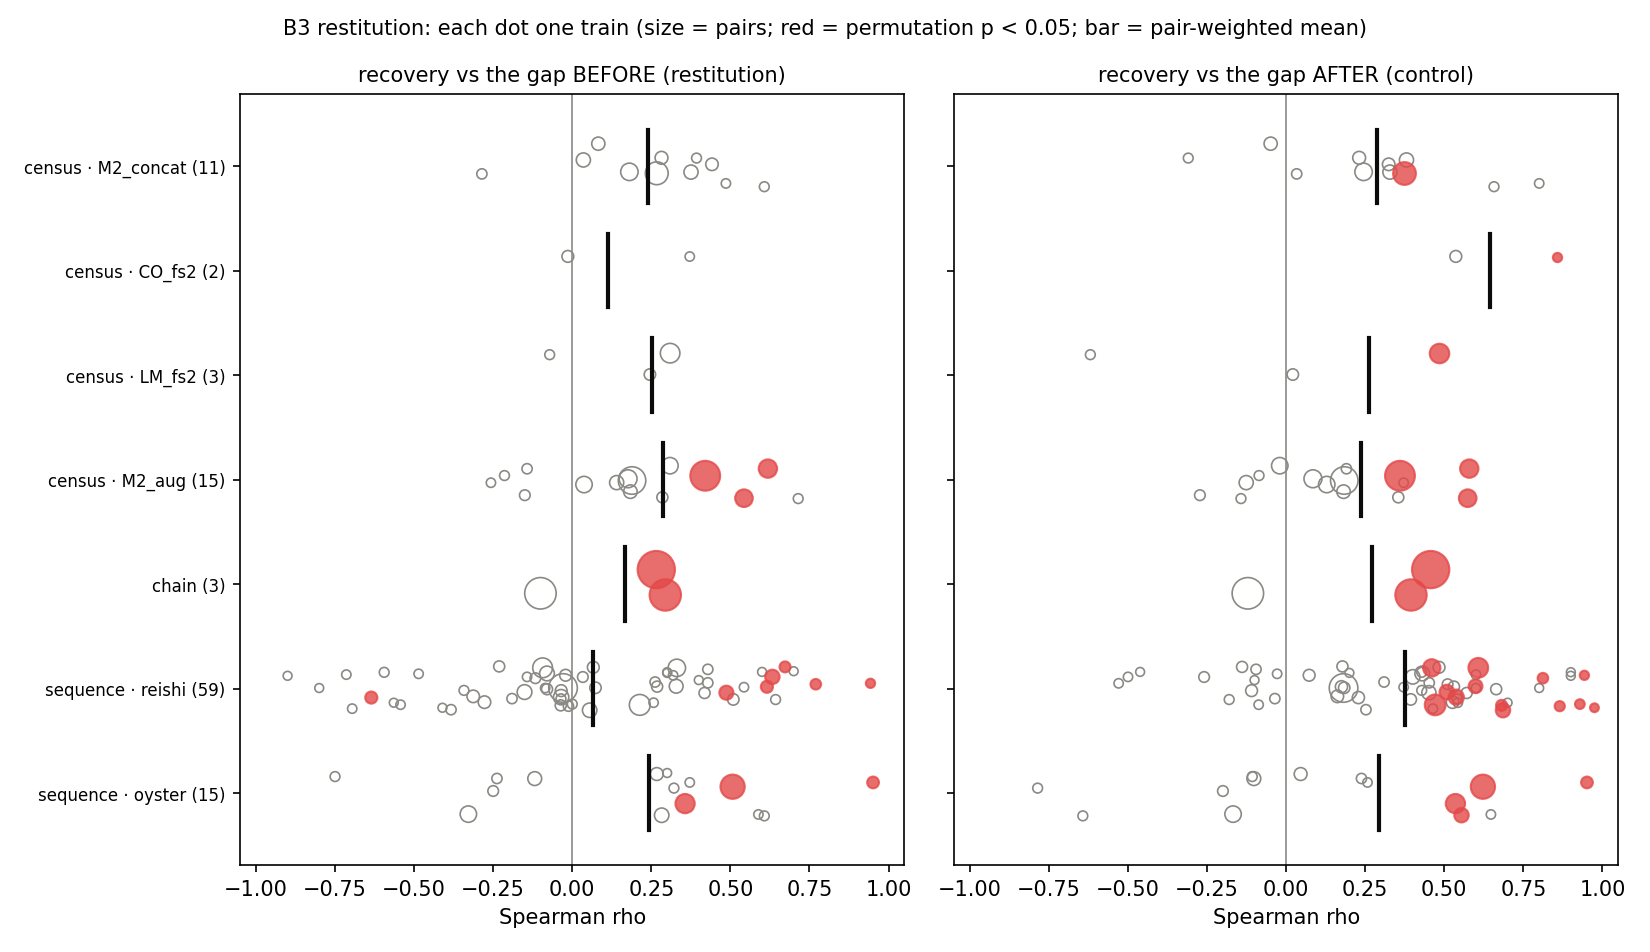
\includegraphics[width=\textwidth]{data/ch10_fhn/b3_restitution_rho.png}
\caption{Restitution. Each dot is one train's Spearman $\rho$ between recovery time and the gap before each drop (left) or the gap after it (right, a control). Dot size is the number of pairs, red marks permutation $p<0.05$, and bars are pair-weighted means. Recovery correlates as strongly with the gap after as with the gap before: a censoring artefact, not restitution.}
\label{fig:b3restitution}
\end{figure}

\begin{figure}[htbp]
\centering
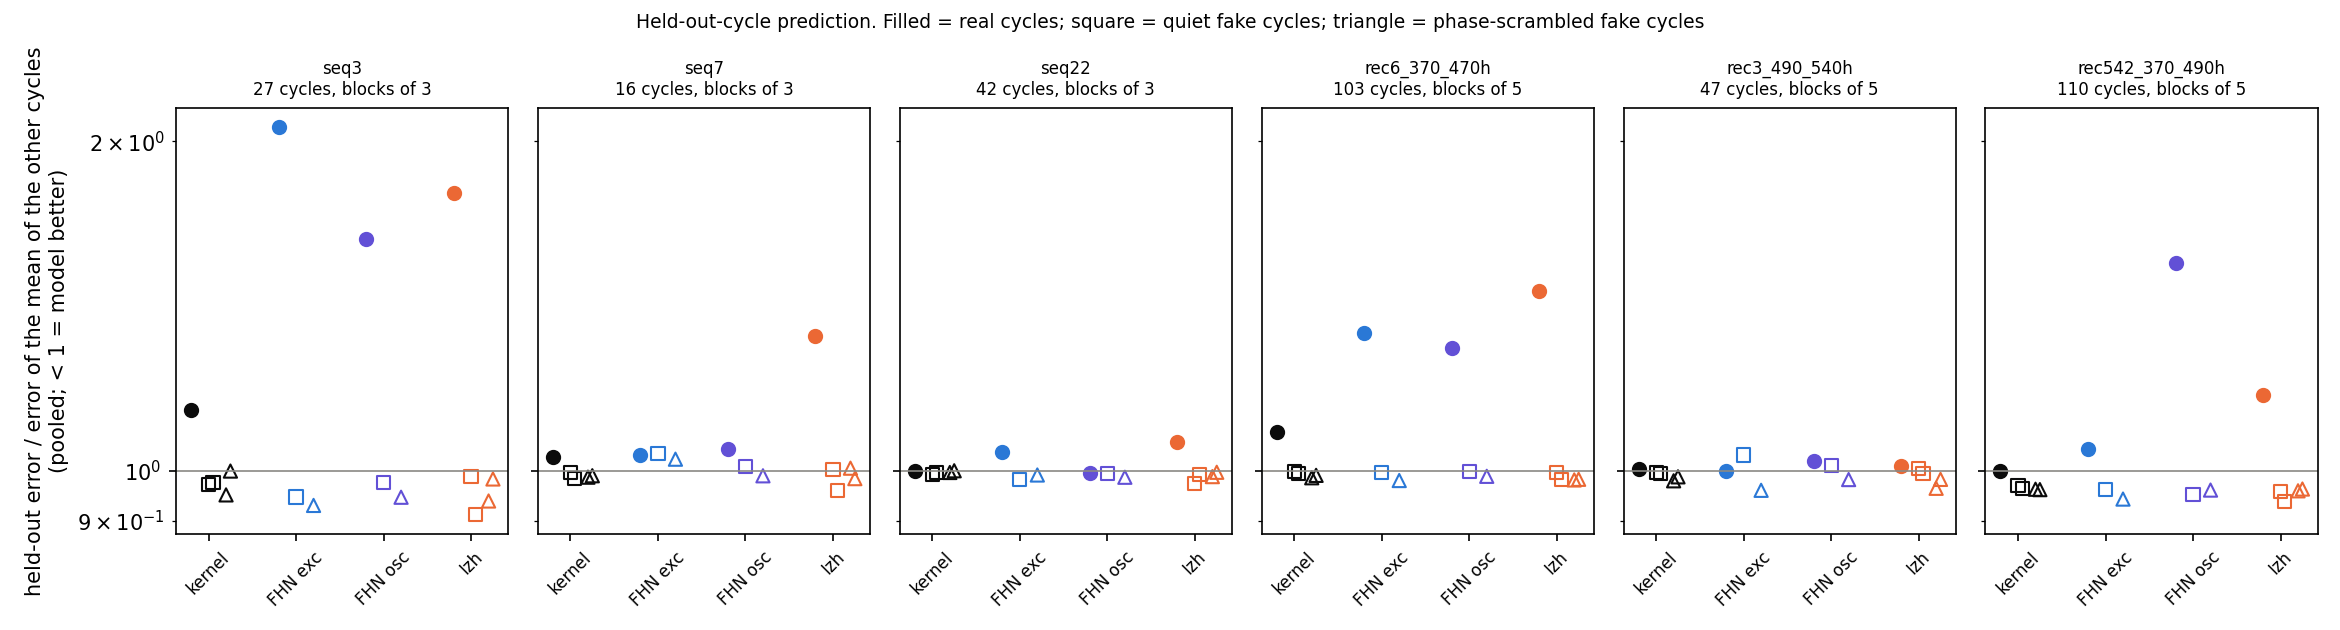
\includegraphics[width=\textwidth]{data/ch10_fhn/b3_track_ratio.png}
\caption{Held-out-cycle prediction. Each model's error on cycles it never saw, divided by the error of the mean of the neighbouring cycles; below 1, the model is better. Filled: real cycles; open: quiet (squares) and phase-scrambled (triangles) fake cycles. No model beats the neighbours' mean on real cycles, and all beat it slightly on fakes.}
\label{fig:b3track}
\end{figure}

\begin{figure}[htbp]
\centering
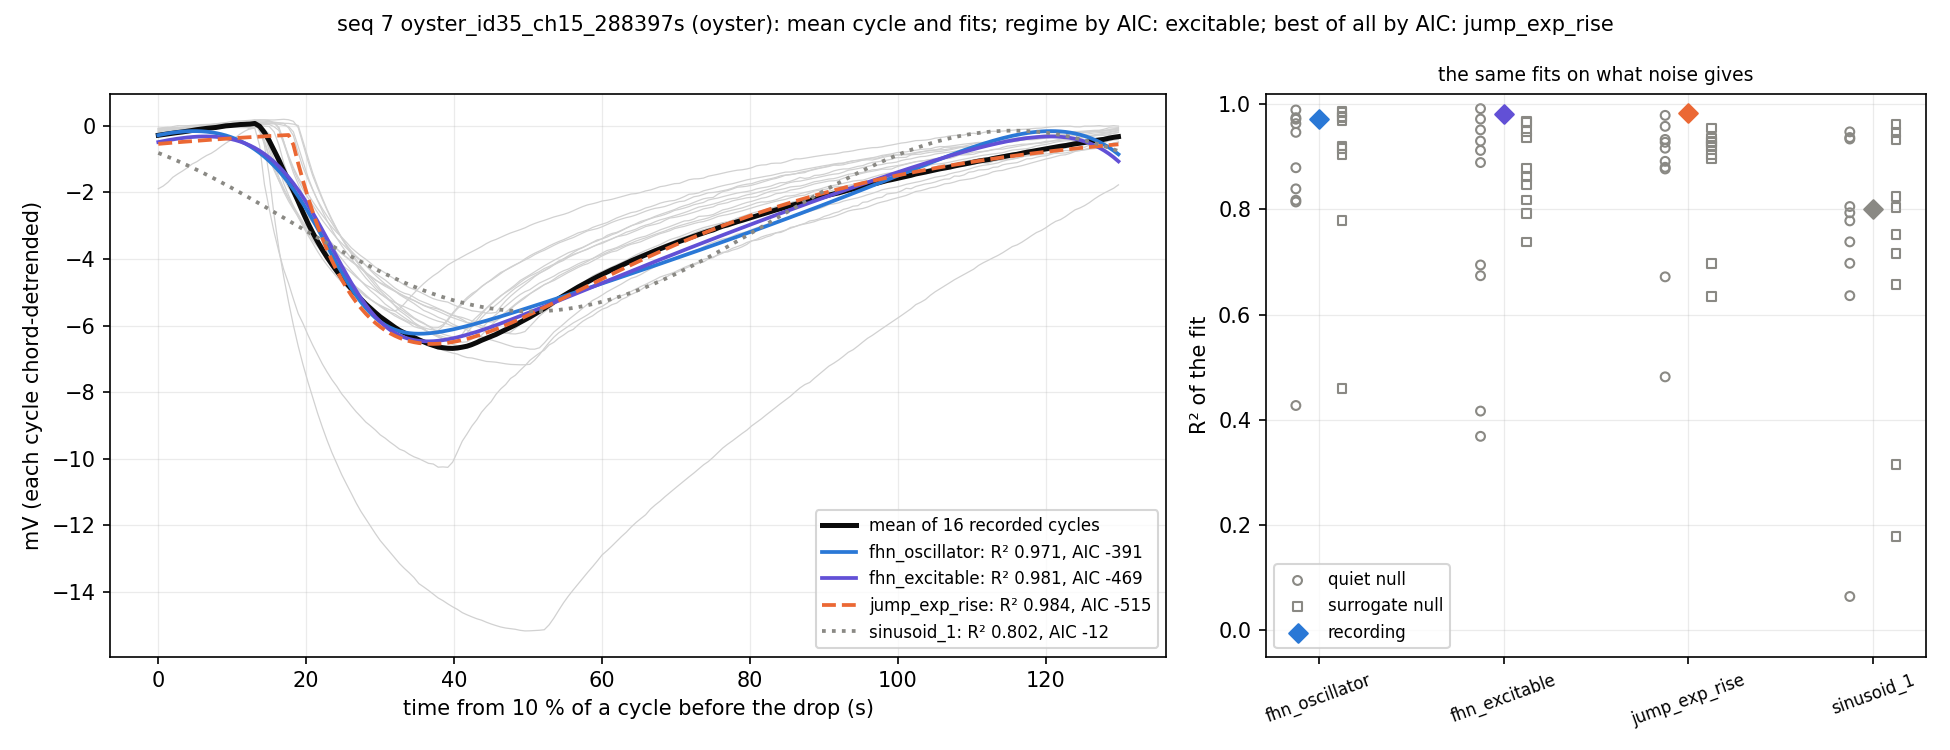
\includegraphics[width=\textwidth]{data/ch10_fhn/seq7_fit.png}
\caption{Oyster sequence 7: the mean of 16 recorded drop cycles with four fitted models (left), and the same fits on quiet-stretch and scrambled fake cycles (right). A fall plus smooth recovery fits best; FHN fits the fakes about as well as the recording.}
\label{fig:fhnfit}
\end{figure}

\begin{figure}[htbp]
\centering
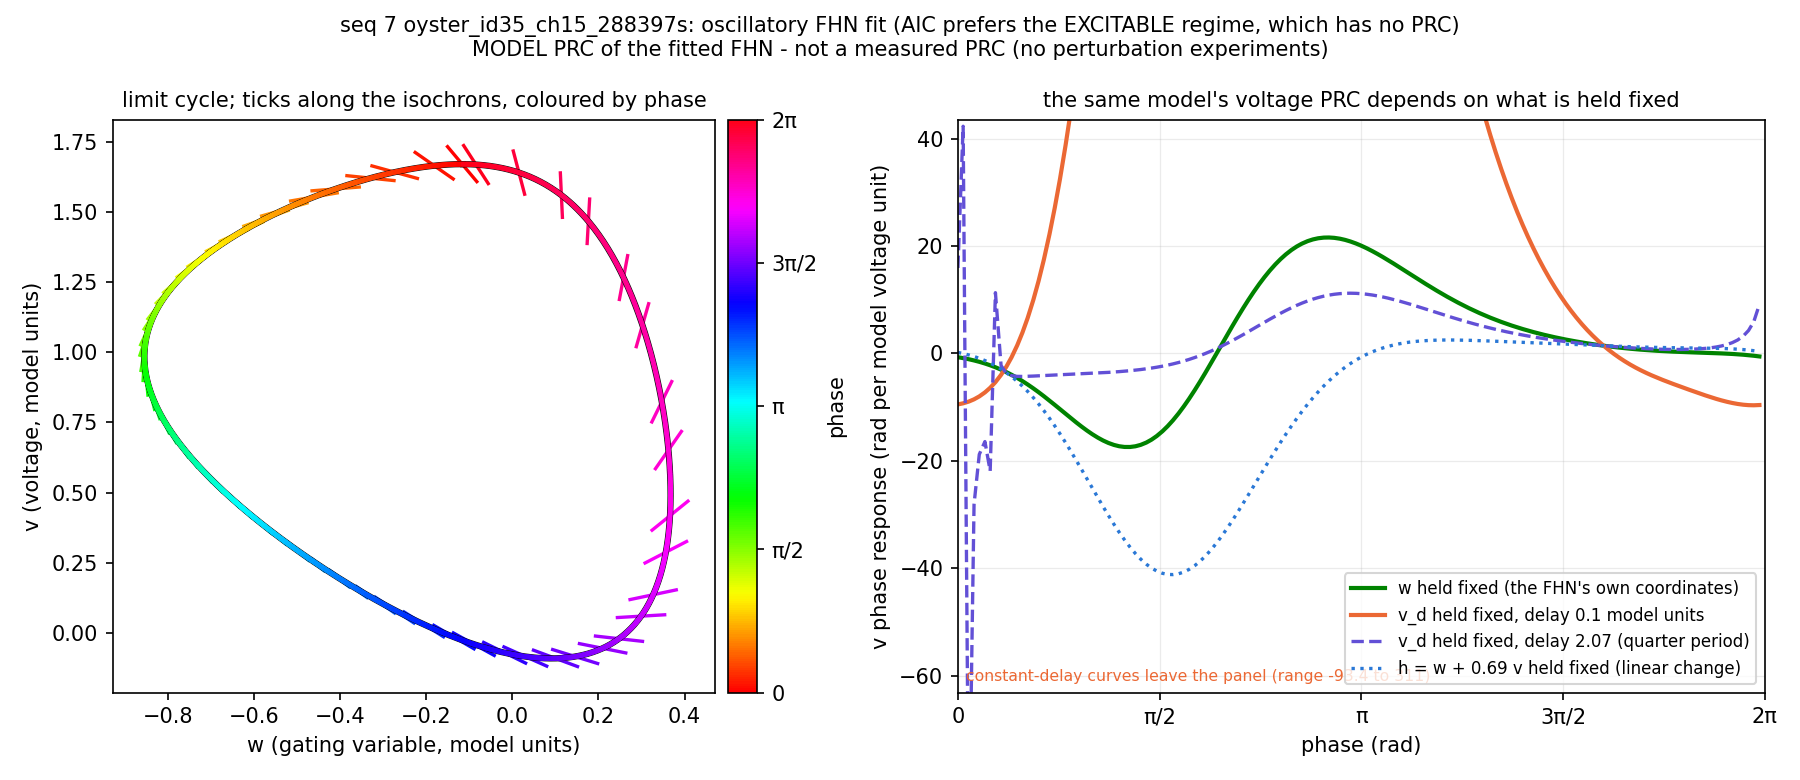
\includegraphics[width=\textwidth]{data/ch10_fhn/seq7_fig1_style.png}
\caption{The oscillatory FHN fitted to sequence 7, drawn in the manner of Wilshin et al.\ \cite{wilshin2024prc}: the limit cycle with phase-coloured isochron ticks (left), and the model's voltage PRC under four choices of what is held fixed (right). This is the PRC of the fitted model, not a measured one.}
\label{fig:fhn}
\end{figure}

